\documentclass[11pt]{article}
\usepackage{amsmath,amsbsy,amssymb,verbatim,fullpage,ifthen,graphicx,bm,amsfonts,amsthm,url}
\usepackage{graphicx}
\usepackage{xcolor}
\newcommand{\mfile}[1]  {{\small \verbatiminput{./#1}}} % Jeff Fessler, input matlab file
\newcommand{\tmop}[1]{\ensuremath{\operatorname{#1}}}
%\newcommand*{\qed}{\hfill\ensuremath{\blacksquare}}%
\newcommand{\R}{\mathbb{R}}
\newcommand{\C}{\mathbb{C}}
\newcommand{\Z}{\mathbb{Z}}
\newcommand{\A}{\mathcal{A}}
\newcommand{\minimize}{\operatorname*{minimize\ }}
\newcommand{\maximize}{\operatorname*{maximize}}
\newcommand{\opdet}[1]{\operatorname{\textbf{det}}\left(#1\right)}
\newcommand{\optr}[1]{\operatorname{\textbf{tr}}\left(#1\right)}
\newcommand{\AnswerDefine}{}
\newcommand{\answer}[2][blue]{\ifdefined\AnswerDefine{\color{#1}\it#2}\fi}
\newcommand{\mtx}[1]{\mathbf{#1}}
\newcommand{\vct}[1]{\mathbf{#1}}
\def \lg       {\langle}
\def \rg       {\rangle}
\def \mA {\mtx{A}}
\def \mB {\mtx{B}}
\def \mD {\mtx{D}}
\def \mE {\mtx{E}}
\def \mF {\mtx{F}}
\def \mG {\mtx{G}}
\def \mI {\mtx{I}}
\def \mJ {\mtx{J}}
\def \mL {\mtx{L}}
\def \mU {\mtx{U}}
\def \mS {\mtx{S}}
\def \mV {\mtx{V}}
\def \mW {\mtx{W}}
\def \mLambda {\mtx{\Lambda}}
\def \mSigma {\mtx{\Sigma}}
\def \mX {\mtx{X}}
\def \mY {\mtx{Y}}
\def \mZ {\mtx{Z}}
\def \zero     {\mathbf{0}}
\def \vzero    {\vct{0}}
\def \vone    {\vct{1}}
\def \va {\vct{a}}
\def \vg {\vct{g}}
\def \vm {\vct{m}}
\def \vu {\vct{u}}
\def \vv {\vct{v}}
\def \vw {\vct{w}}
\def \vx {\vct{x}}
\def \vy {\vct{y}}
\def \vz {\vct{z}}
\def \vphi {\vct{\phi}}
\def \vmu {\vct{\mu}}
\def \R {\mathbb{R}}

%\newcommand{\st}{\operatorname*{\ subject\ to\ }}
\usepackage{algorithm,algpseudocode}
\usepackage{xspace}
\usepackage{mathtools} 
\usepackage{amsmath}
% Add a period to the end of an abbreviation unless there's one
% already, then \xspace.
\makeatletter
\DeclareRobustCommand\onedot{\futurelet\@let@token\@onedot}
\def\@onedot{\ifx\@let@token.\else.\null\fi\xspace}

\def\eg{\emph{e.g}\onedot} \def\Eg{\emph{E.g}\onedot}
\def\ie{\emph{i.e}\onedot} \def\Ie{\emph{I.e}\onedot}
\def\cf{\emph{c.f}\onedot} \def\Cf{\emph{C.f}\onedot}
\def\etc{\emph{etc}\onedot} \def\vs{\emph{vs}\onedot}
\def\wrt{w.r.t\onedot} \def\dof{d.o.f\onedot}
\def\etal{\emph{et al}\onedot} \def\st{\emph{s.t}\onedot}
\pagestyle{plain}
\usepackage{listings}
\usepackage{color} %red, green, blue, yellow, cyan, magenta, black, white
\definecolor{mygreen}{RGB}{28,172,0} % color values Red, Green, Blue
\definecolor{mylilas}{RGB}{170,55,241}
\lstset{language=Matlab,%
    %basicstyle=\color{red},
    breaklines=true,%
    morekeywords={matlab2tikz},
    keywordstyle=\color{blue},%
    morekeywords=[2]{1}, keywordstyle=[2]{\color{black}},
    identifierstyle=\color{black},%
    stringstyle=\color{mylilas},
    commentstyle=\color{mygreen},%
    showstringspaces=false,%without this there will be a symbol in the places where there is a space
    numbers=left,%
    numberstyle={\tiny \color{black}},% size of the numbers
    numbersep=9pt, % this defines how far the numbers are from the text
    emph=[1]{for,end,break},emphstyle=[1]\color{red}, %some words to emphasise
    %emph=[2]{word1,word2}, emphstyle=[2]{style},    
}

\title{{\bf Final Exam, CPSC 8420, Spring 2022}} 
\author{\Large\underline{Sherrer, Will}}% put your name in the LastName, FirstName format
\date{\textbf{\Large\textcolor{red}{Due 05/06/2022, Friday, 11:59PM EST}}} 
%\date{\today}

\begin{document}
\maketitle

\section*{Problem 1 [15 pts]}
Consider the elastic-net optimization problem:
\begin{equation}
\min_{\beta} \|\vy-\mX\beta\|^2+\lambda[\alpha\|\beta\|^2_2+(1-\alpha)\|\beta\|_1].
\end{equation}
\begin{enumerate}
	\item Show the objective can be reformulated into a lasso problem, with a slightly different $\mX, \vy$.\\
	
	We can see that if alpha is 0, the ridge regression aspect of elastic net will go to 0 and we will have the Lasso formulation remaining as
\begin{equation}
\min_{\beta} \|\vy-\mX\beta\|^2+\lambda\|\beta\|_1
\end{equation}
	\item If we fix $\alpha=.5$, please derive the closed solution by making use of alternating minimization that each time we fix the rest by optimizing one single element in $\beta$. You need randomly generate $\mX, \vy$ and initialize  $\beta_0$, and show the objective decreases monotonically with updates.\\\\

First we can use reformulate the objective with $\alpha$ = 0.5 to be: 
\begin{equation}
\min_{\beta} \|\vy-\mX\beta\|^2+ \frac{\lambda}{2}\|\beta\|^2_2+\frac{\lambda}{2}\|\beta\|_1.
\end{equation}
We can take the derivative w.r.t $\beta$, however since we are also using L1 norm, we must divide into positive and negative cases where:
$\hat{\beta} = -2*X^T(y - X\beta) + \frac{\lambda}{2} \beta$\\
\begin{equation}
\hat{\beta}^{Lasso} = \left\{ \begin{array}{ll}
            \hat{\beta} - \frac{\lambda}{2} &  iff \hat{\beta} > \lambda\\
            \hat{\beta} + \frac{\lambda}{2} &  iff \hat{\beta} \leq \lambda\\
            0 & else
        \end{array} \right.
\end{equation}\\
For my implementation I am also randomly initializing $\beta$ and calculating for 100 iterations with a learning rate of $0.0001$ and where $\lambda$ = 1.Since I am not plotting the objective with different $\lambda$ since I only need to show that the objective is decreasing. \\
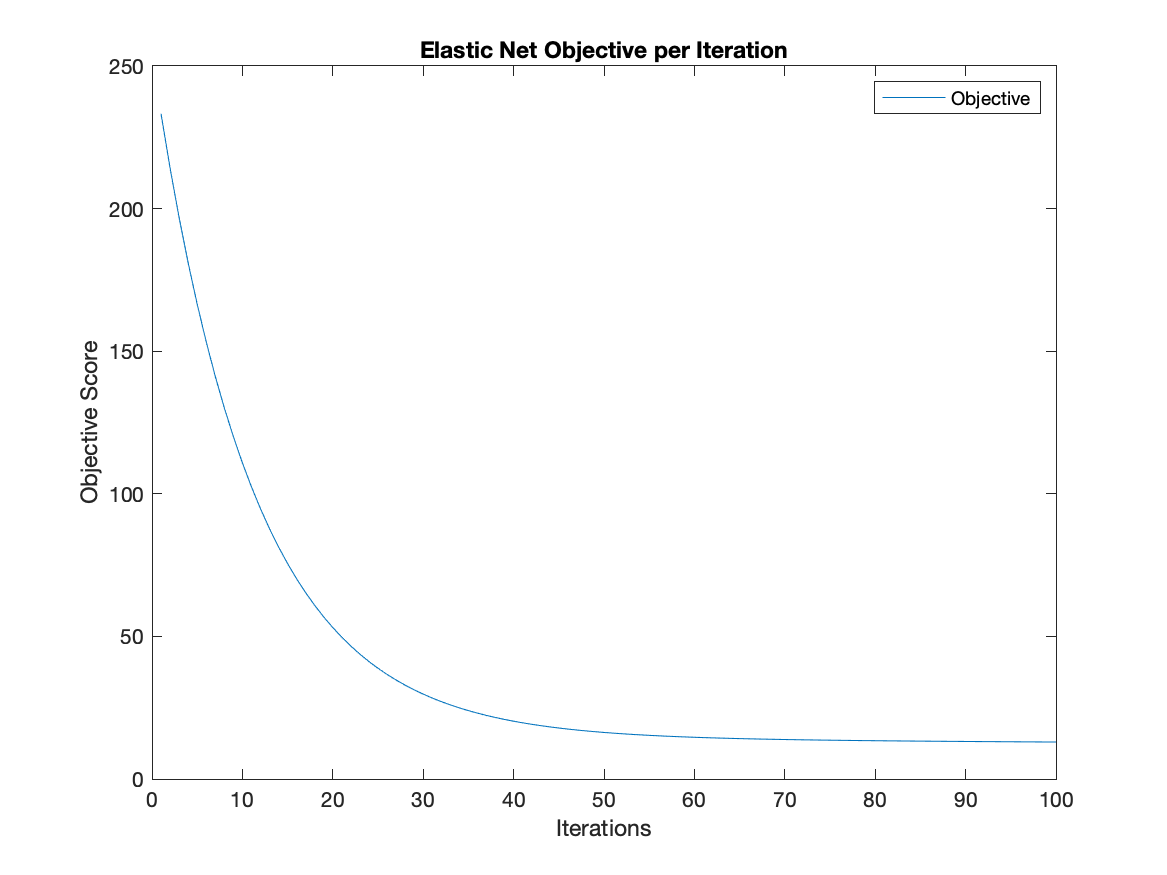
\includegraphics[scale=.95]{elastic_net_ob.png}\\
From this graph I can see that the objective of Elastic Net Objective is decreasing per iteration.
\end{enumerate}


\newpage
\section*{Problem 2 [15 pts]}
\begin{itemize}
	\item For PCA, the loading vectors can be directly computed from the $q$ columns of  $\mU$ where  $[\mU,\mS,\mU]=svd(\mX^T\mX)$, please show that any $[\pm\vu_1,\pm\vu_2,\dots,\pm\vu_q]$ will be equivalent to $[\vu_1,\vu_2,\dots,\vu_q]$ in terms of the same variance while satisfying the orthonormality constraint.\\\\
	We know that the columns of U are orthogonal as that is in the definition of SVD. Orthogonal vectors are calculated by taking the dot product which takes the cosine of the angle between the vectors. Cosine has a symmetrical property and is an even function meaning that $cos(\theta) = cos(-\theta)$. Since the magnitude is not dependent of the signs of the vector, and the angle between the vectors is the same whether negative or positve, the dot product of both positive and negative columns will be the same which is 0. This means negative columns of U satisfies the orthonormality constraint. 
	
We can assume that $\phi = \sum^p_{i=1} \lambda_i U(:, i)$ and the constraint $||\phi||_2 = 1$ is equal to $\sum^p_{i=1} \lambda_i^2 = 1$. We can rewrite $X^TX = \sum^p_{i=1} S(i, i)U(:,i)U(:,i)^T$ and since we know the columns of U are orthogonal whether negative or positive, therefore, $||X\phi||_2^2 = \sum^p_{i=1} S(i,i)\lambda_i^2 \le S(1,1)$ Therefore the variance is the same in both cases. 

	\item We consider the case when original dimensionality of the data is much larger than the number of samples $d\gg m$ ($\mX\in\R^{d\times m}$). What's the complexity of obtaining the optimal solution of PCA via Singular Value Decomposition? Please consider a more efficient solution by considering the relationships of eigenvalues/eigenvectors between $\mX^T\mX$ and $\mX\mX^T$.\\\\
	I found that the time complexity of SVD is$O(n^3)$. In a d x m matrix when d$\gg$m, we want to use $X^TX$ so that we are performing SVD on an m x m matrix.\\\\
	For matrix $X$ of size $m x n$, We can show that both $X^TX and XX^T$ are symmetric square matrices of size (n, n) and (m, m), respectively.\\\\
	$(X^TX)^T = X^T (X^T)^T = X^TX$\\
	$(XX^T)^T = (X^T)^T X^T = XX^T$\\\\
	It can also be shown that $XX^T$ and $X^TX$ share the same non-zero eigenvalues. If one has more eigenvalues than the other, all of the excess eigenvalues should be zero.\\
	If we let $v$ = the eigenvector of $X^TX$ and $\lambda$ be its eigenvalue:\\
	$X^TXb = \lambda v$ -- if we multiply both sides by $X$ then:\\
	$XX^T (Xv) = \lambda (X v)$.\\ Since $\lambda$ does not = 0, it follows $X^T v$ does not = 0, therefore $X^T v$ is an eigenvector of $X^TX$ with eigenvalue of $\lambda$\\
	The eigenvectors to eigenvalue zero are the elements in the null space of $X: X^T v = 0$ implies $v^TX^TXv = ||Xv||^2 = 0$, which is $Xv$=0. You obtain the eigenvectors of $X^TX$ from $X^Tv$  with $v$ eigenvector of $v$ of $XX^T$ to non-zero eigenvalue. Therefore you can obtain $V$ , whose each column is an eigenvector for $XX^T$, and D, a diagonal matrix holding $XX^T$'s eigenvalues.
\end{itemize}


\newpage
\section*{Problem 3 [10 pts]}
Assume that in a community, there are $10\%$ people suffer from COVID. Assume $80\%$ of the patients come to breathing difficulty while $25\%$ of those free from COVID also have symptoms of shortness of breath. Now please determine that if one has breathing difficulty, what's his/her probability to get COVID? (\textit{hint}: you may consider Naive Bayes)\\

\noindent I want to calculate the probability of getting covid given that they have breathing difficulty. P(C\(|\)B).\\\\
I say that the probability of getting covid, P(C) is 0.1. 
The probability of having difficulty breathing given that they have covid is P(B$|$C) = 0.8.\\

\noindent To calculate the probability that one has breathing difficulty, I need to add the probability of breathing difficulty given covid and without covid. \\

\noindent P(B) = P(B$|$C) * P(C) + P(B$|\bar{C}$) * P($\bar{C}$)\\
P(B) = 0.8 * 0.1 + 0.25 * 0.9\\
P(B) = .08 + .225 = .305\\


\noindent P(C\(|\)B) = $\frac{P(B|C) * P(C)}{P(B)}$ = $\frac{0.8 * 0.1}{0.305}$ = $\frac{0.08}{0.305}$ = 0.2623 or 26.23\%


\newpage
\section*{Problem 4 [20 pts]}
Recall the objective for \text{RatioCut}: $RatioCut(A_1,A_2,...A_k) = \frac{1}{2}\sum\limits_{i=1}^{k}\frac{W(A_i, \overline{A}_i )}{|A_i|}$. If we introduce indicator vector: $h_j \in \{h_1, h_2,..h_k\}, j \in [1,k]$, for any vector $h_j\in R^n$, we define: $h_{ij}= \begin{cases} 0& { v_i \notin A_j}\\ \frac{1}{\sqrt{|A_j|}}& { v_i \in A_j} \end{cases}$, we can prove: $h_i^TLh_i =  \frac{cut(A_i, \overline{A}_i)}{|A_i|}$, and therefore:
\begin{equation}
	RatioCut(A_1,A_2,...A_k) = \sum\limits_{i=1}^{k}h_i^TLh_i = \sum\limits_{i=1}^{k}(H^TLH)_{ii} = tr(H^TLH),
\end{equation}
thus we relax it as an optimization problem:
\begin{equation}
	\underbrace{arg\;min}_H\; tr(H^TLH) \;\; s.t.\;H^TH=I.
\end{equation}
Now let's explore Ncut, with objective:
$NCut(A_1,A_2,...A_k) = \frac{1}{2}\sum\limits_{i=1}^{k}\frac{W(A_i, \overline{A}_i )}{vol(A_i)}$, where $vol(A): = \sum\limits_{i \in A}d_i, d_i: = \sum\limits_{j=1}^{n}w_{ij}$.Similar to Ratiocut, we define: $h_{ij}= \begin{cases} 0& { v_i \notin A_j}\\ \frac{1}{\sqrt{vol(A_j)}}& { v_i \in A_j} \end{cases}$. Now
\begin{enumerate}
	\item Please show that $h_i^TLh_i =\frac{cut(A_i, \overline{A}_i)}{vol(A_i)}$.\\
	$h_i^TLh_i = \frac{1}{2}\displaystyle\sum_{m=1}\displaystyle\sum_{n=1}w_{mn}(h_{im} - h_{in})^2$\\
	$= \frac{1}{2}( \displaystyle\sum_{m \in A_i, n \notin A_i} w_{mn}(\frac{1}{\sqrt{vol(A_i)}} - 0)^2 + \displaystyle\sum_{m \notin A_i, n \in A_i} w_{mn}(0 - \frac{1}{\sqrt{vol(A_i)}})^2)$\\
	$= \frac{1}{2}( \displaystyle\sum_{m \in A_i, n \notin A_i} w_{mn}\frac{1}{vol(A_i)} + \displaystyle\sum_{m \notin A_i, n \in A_i} w_{mn}\frac{1}{vol(A_i)})$\\
	$=\frac{1}{2}(cut(A_i, \bar{A_i})\frac{1}{vol(A_i)} + cut(\bar{A_i},A_i)\frac{1}{vol(A_i)})$\\
	$= \frac{cut(A_i, \bar{A_i})}{vol(A_i)}$
	\item Show that $NCut(A_1,A_2,...A_k) = tr(H^TLH)$.\\
	Since we have proved $h_i^TLh_i =\frac{cut(A_i, \overline{A}_i)}{vol(A_i)}$, therefore
	\begin{equation}
	NCut(A_1,A_2,...A_k) = \sum\limits_{i=1}^{k}h_i^TLh_i = \sum\limits_{i=1}^{k}(H^TLH)_{ii} = tr(H^TLH),
	\end{equation}
	\item The constraint now is: $H^TDH=I$.
	\item Find the solution to $\underbrace{arg\;min}_H\; tr(H^TLH) \;\; s.t.\;H^TDH=I$.\\
	In Spectural Clustering we need to construct the Laplacian for the obtained graph and
calculate the first k eigenvectors of the Laplacian. The value of k is fixed based on the number of clusters required. We can consider the normalized Laplacian where $L = I - D^{-1}W$. Therefor for $k$ clusters, the solution can be achieved by taking the first $k$ eigenvectors of $I - D^{-1}W$ as the columns of $H$.
\end{enumerate}

\newpage
\section*{Problem 5 [10 pts]}
We consider the following optimization problem ($\mY$ is given and generated randomly):
\begin{equation}
	\min_{\mX} \frac{1}{2}\|\mX-\mY\|^2_F + \|\mX\|_*
\end{equation}
where $\mY,\mX\in\R^{100\times100}$ and $\|\cdot\|_*$ denotes the nuclear norm (sum of singular values). Now please use gradient descent method to update $\mX$. ($\frac{\partial \|\mX\|_*}{\partial \mX}=\mU\mV^T$, where $\mU,\mV$ is obtained from reduced SVD, namely $[\mU,\mS,\mV]=svd(\mX,0)$). Plot the objective changes with 1000 iteration.\\\\
I first noticed that the optimization problem can be rewritten as $tr((X - Y)^T(X - Y))+ \|\mX\|_*$ In which the gradient $w.r.t. X$ can be seen as just being the gradient $(X - Y)$ plus the nuclear norm gradient which is given as $\frac{\partial \|\mX\|_*}{\partial \mX}=\mU\mV^T$. Through a web search on Matlab, I found that calculating the nuclear norm is as follows, $nucnorm = norm(svd(X),1);$ In my code I used a lambda of .001.\\
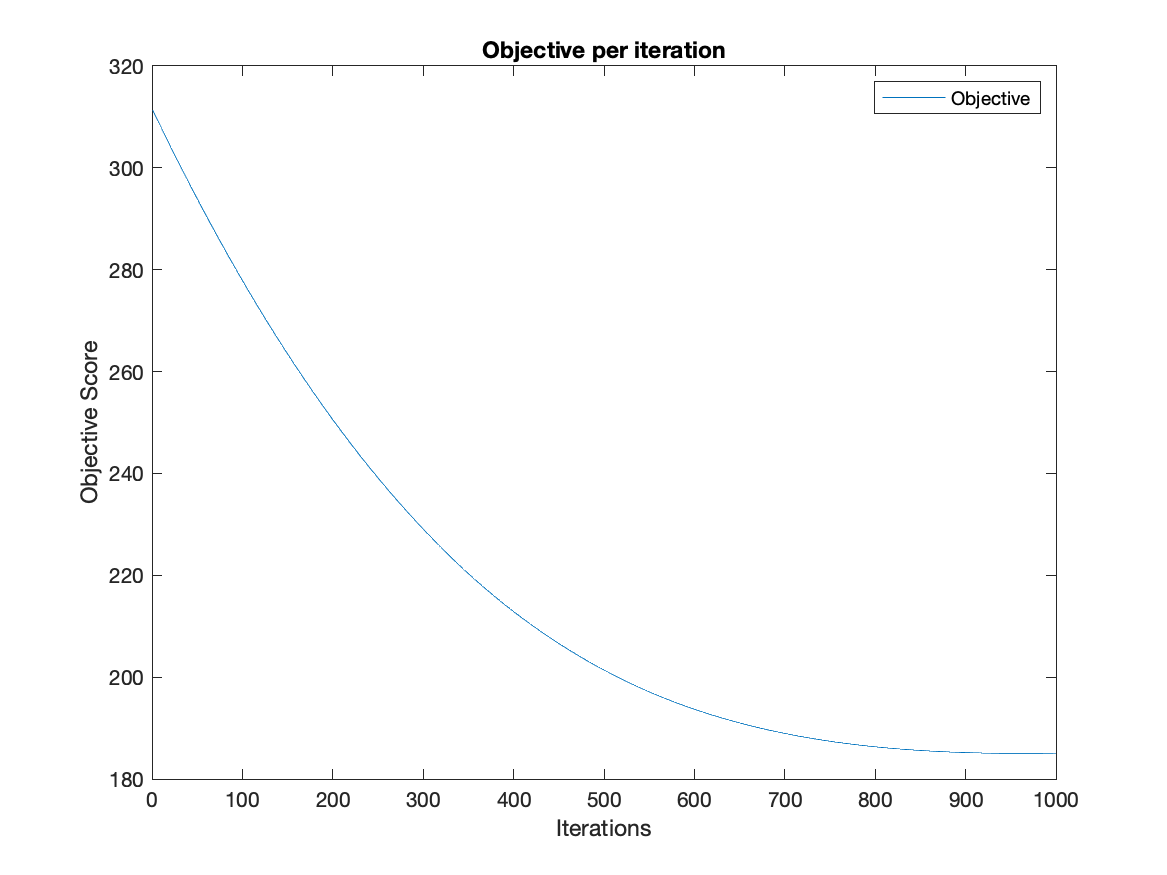
\includegraphics[scale=1]{ob_min.png}

\newpage
\section*{Problem 6 [20 pts]}
We turn to Logistic Regression:
\begin{equation}
	\min_\beta \sum\limits_{i=1}^{m} ln(1+e^{\lg \beta, \hat{x_i}\rg})-y_{i}\lg \beta, \hat{x_i}\rg, 
\end{equation}
where $\beta=(w;b), \hat{x}=(x;1)$. Assume $m=100, x\in\R^{99}$. Please randomly generate $x, y$ and find the optimal $\beta$ via 1) gradient descent; 2) Newton's method and 3) stochastic gradient descent (SGD) where the batch-size is 1. (need consider choosing appropriate  step-size if necessary). Change $m=1000, x\in\R^{999}$, observe which algorithm will decrease the objective faster in terms of iteration ($X$-axis denotes number of iteration) and CPU time. [You will receive another 5 bonus points if you implement backtracking line search]\\

\begin{tabular}{c c}
Norm of the matrix per iteration\\
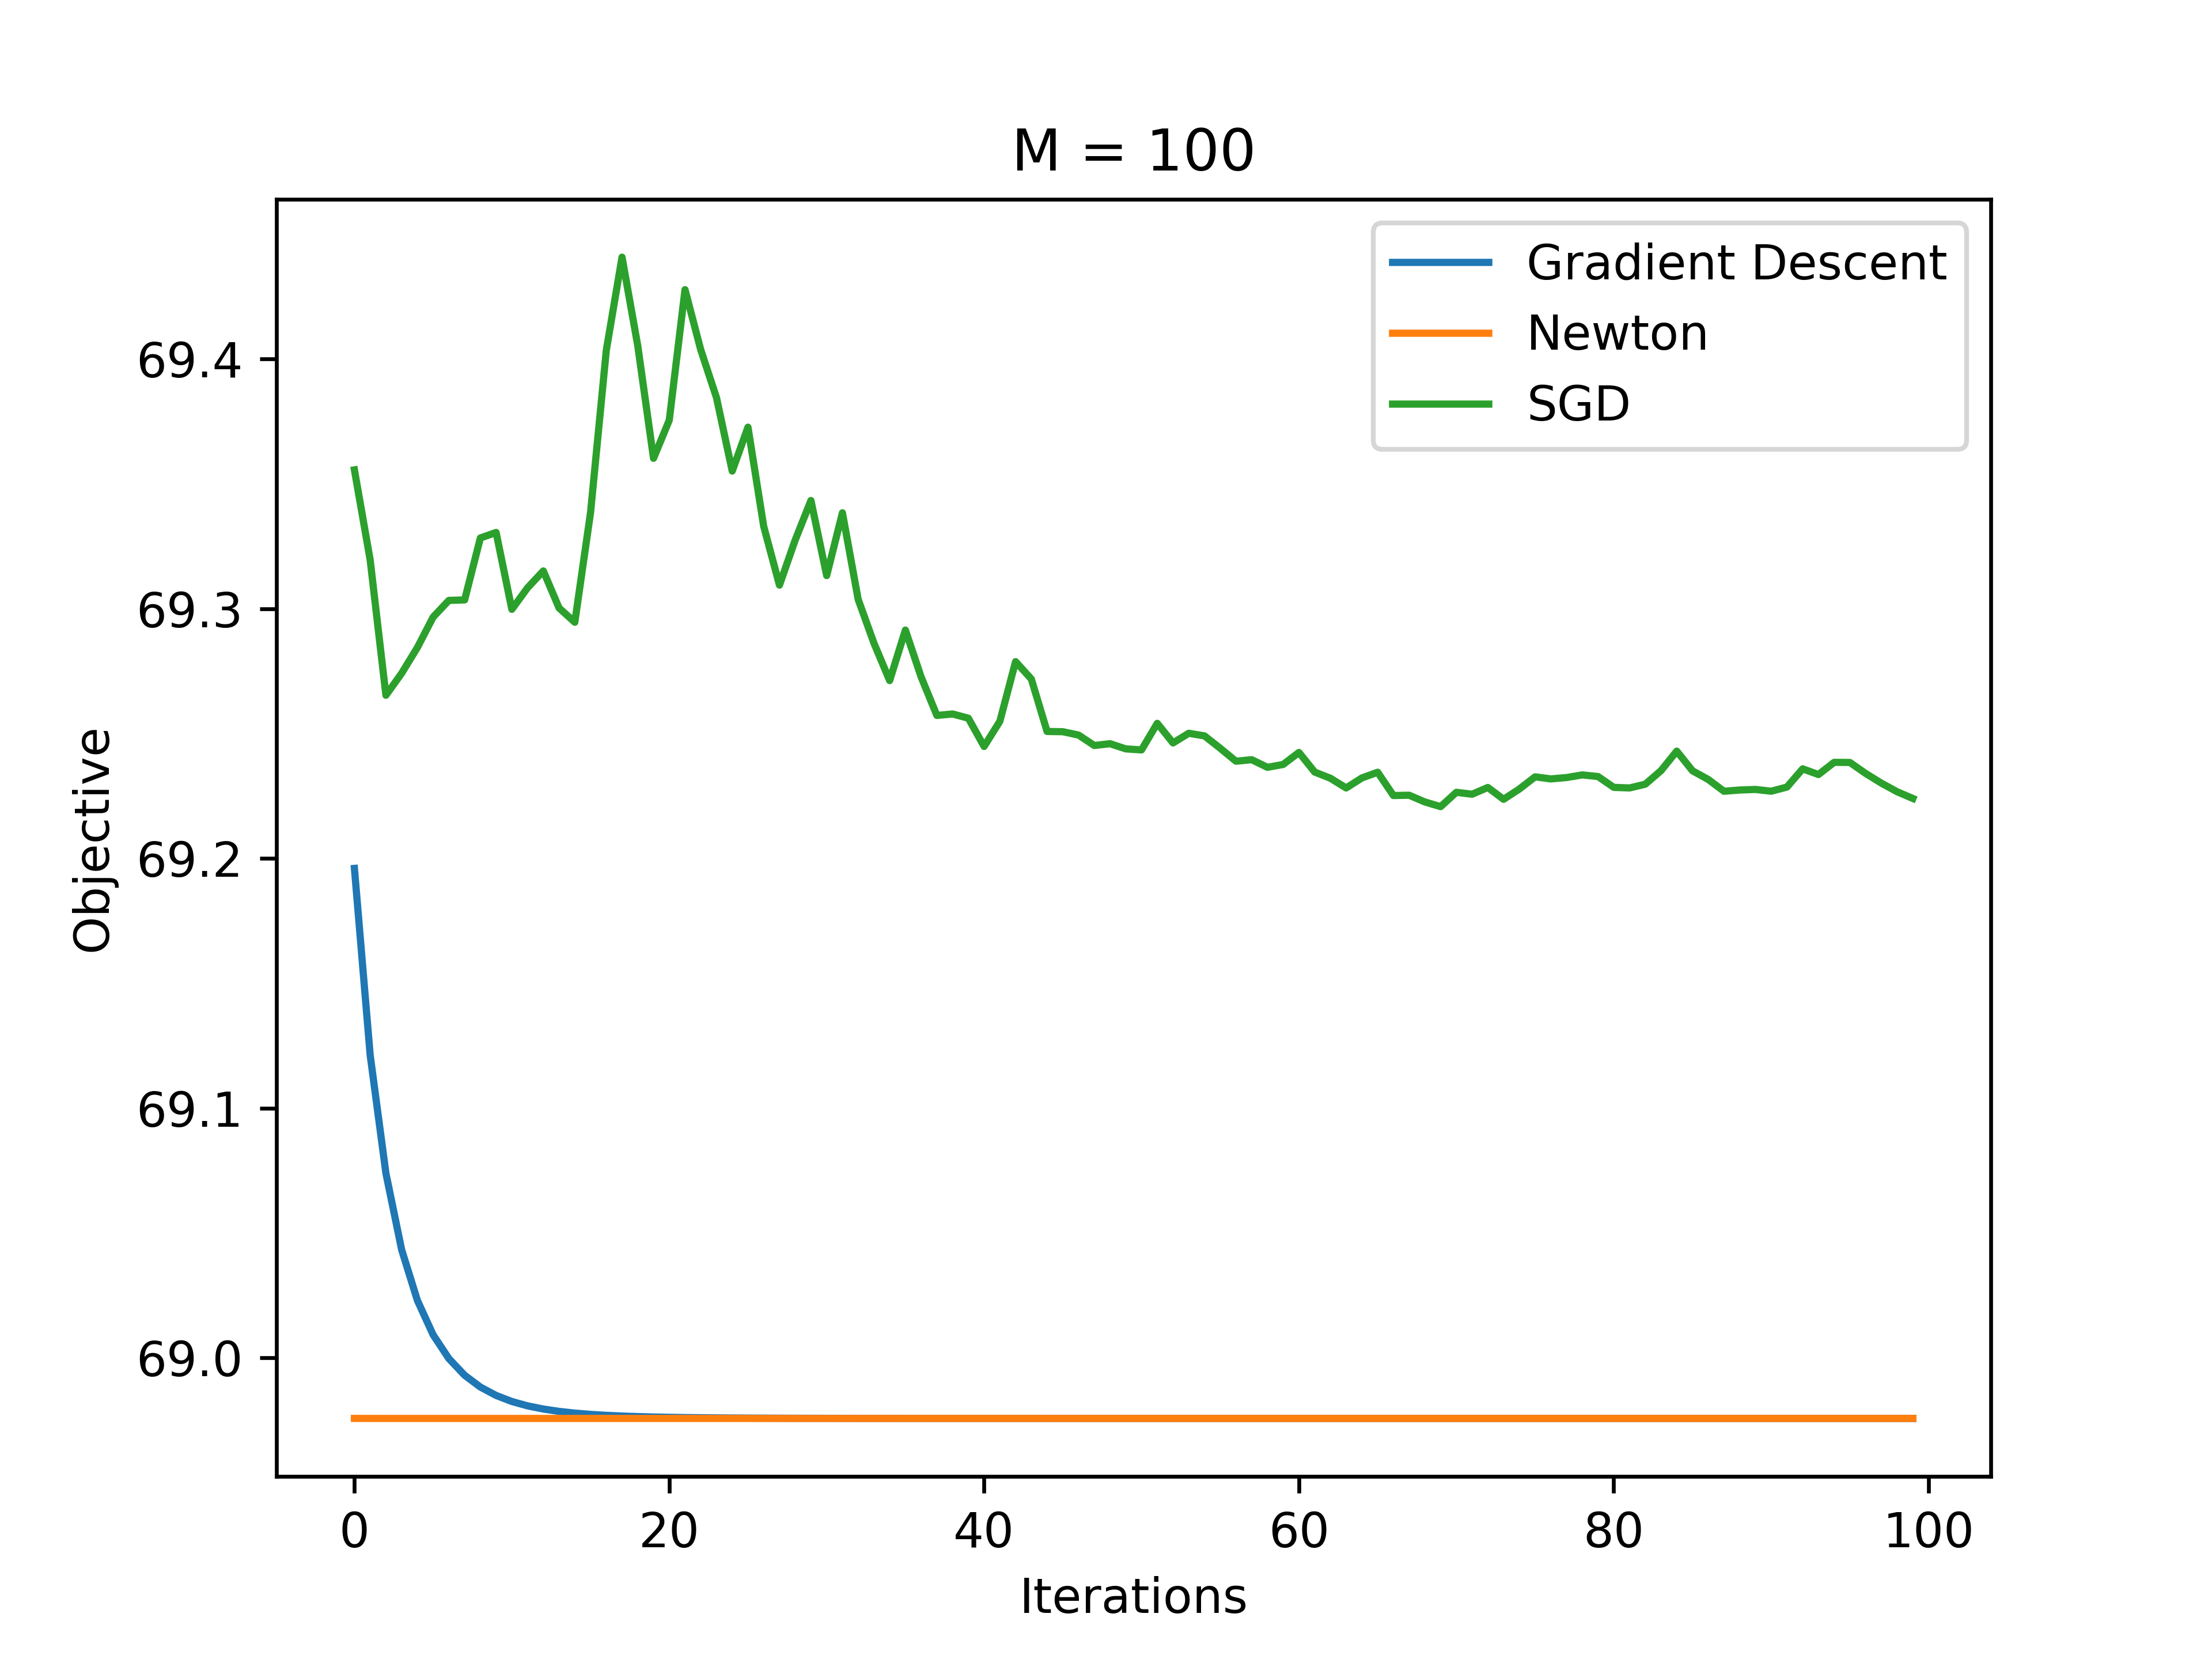
\includegraphics[scale=.55]{norm_m_100.png} & 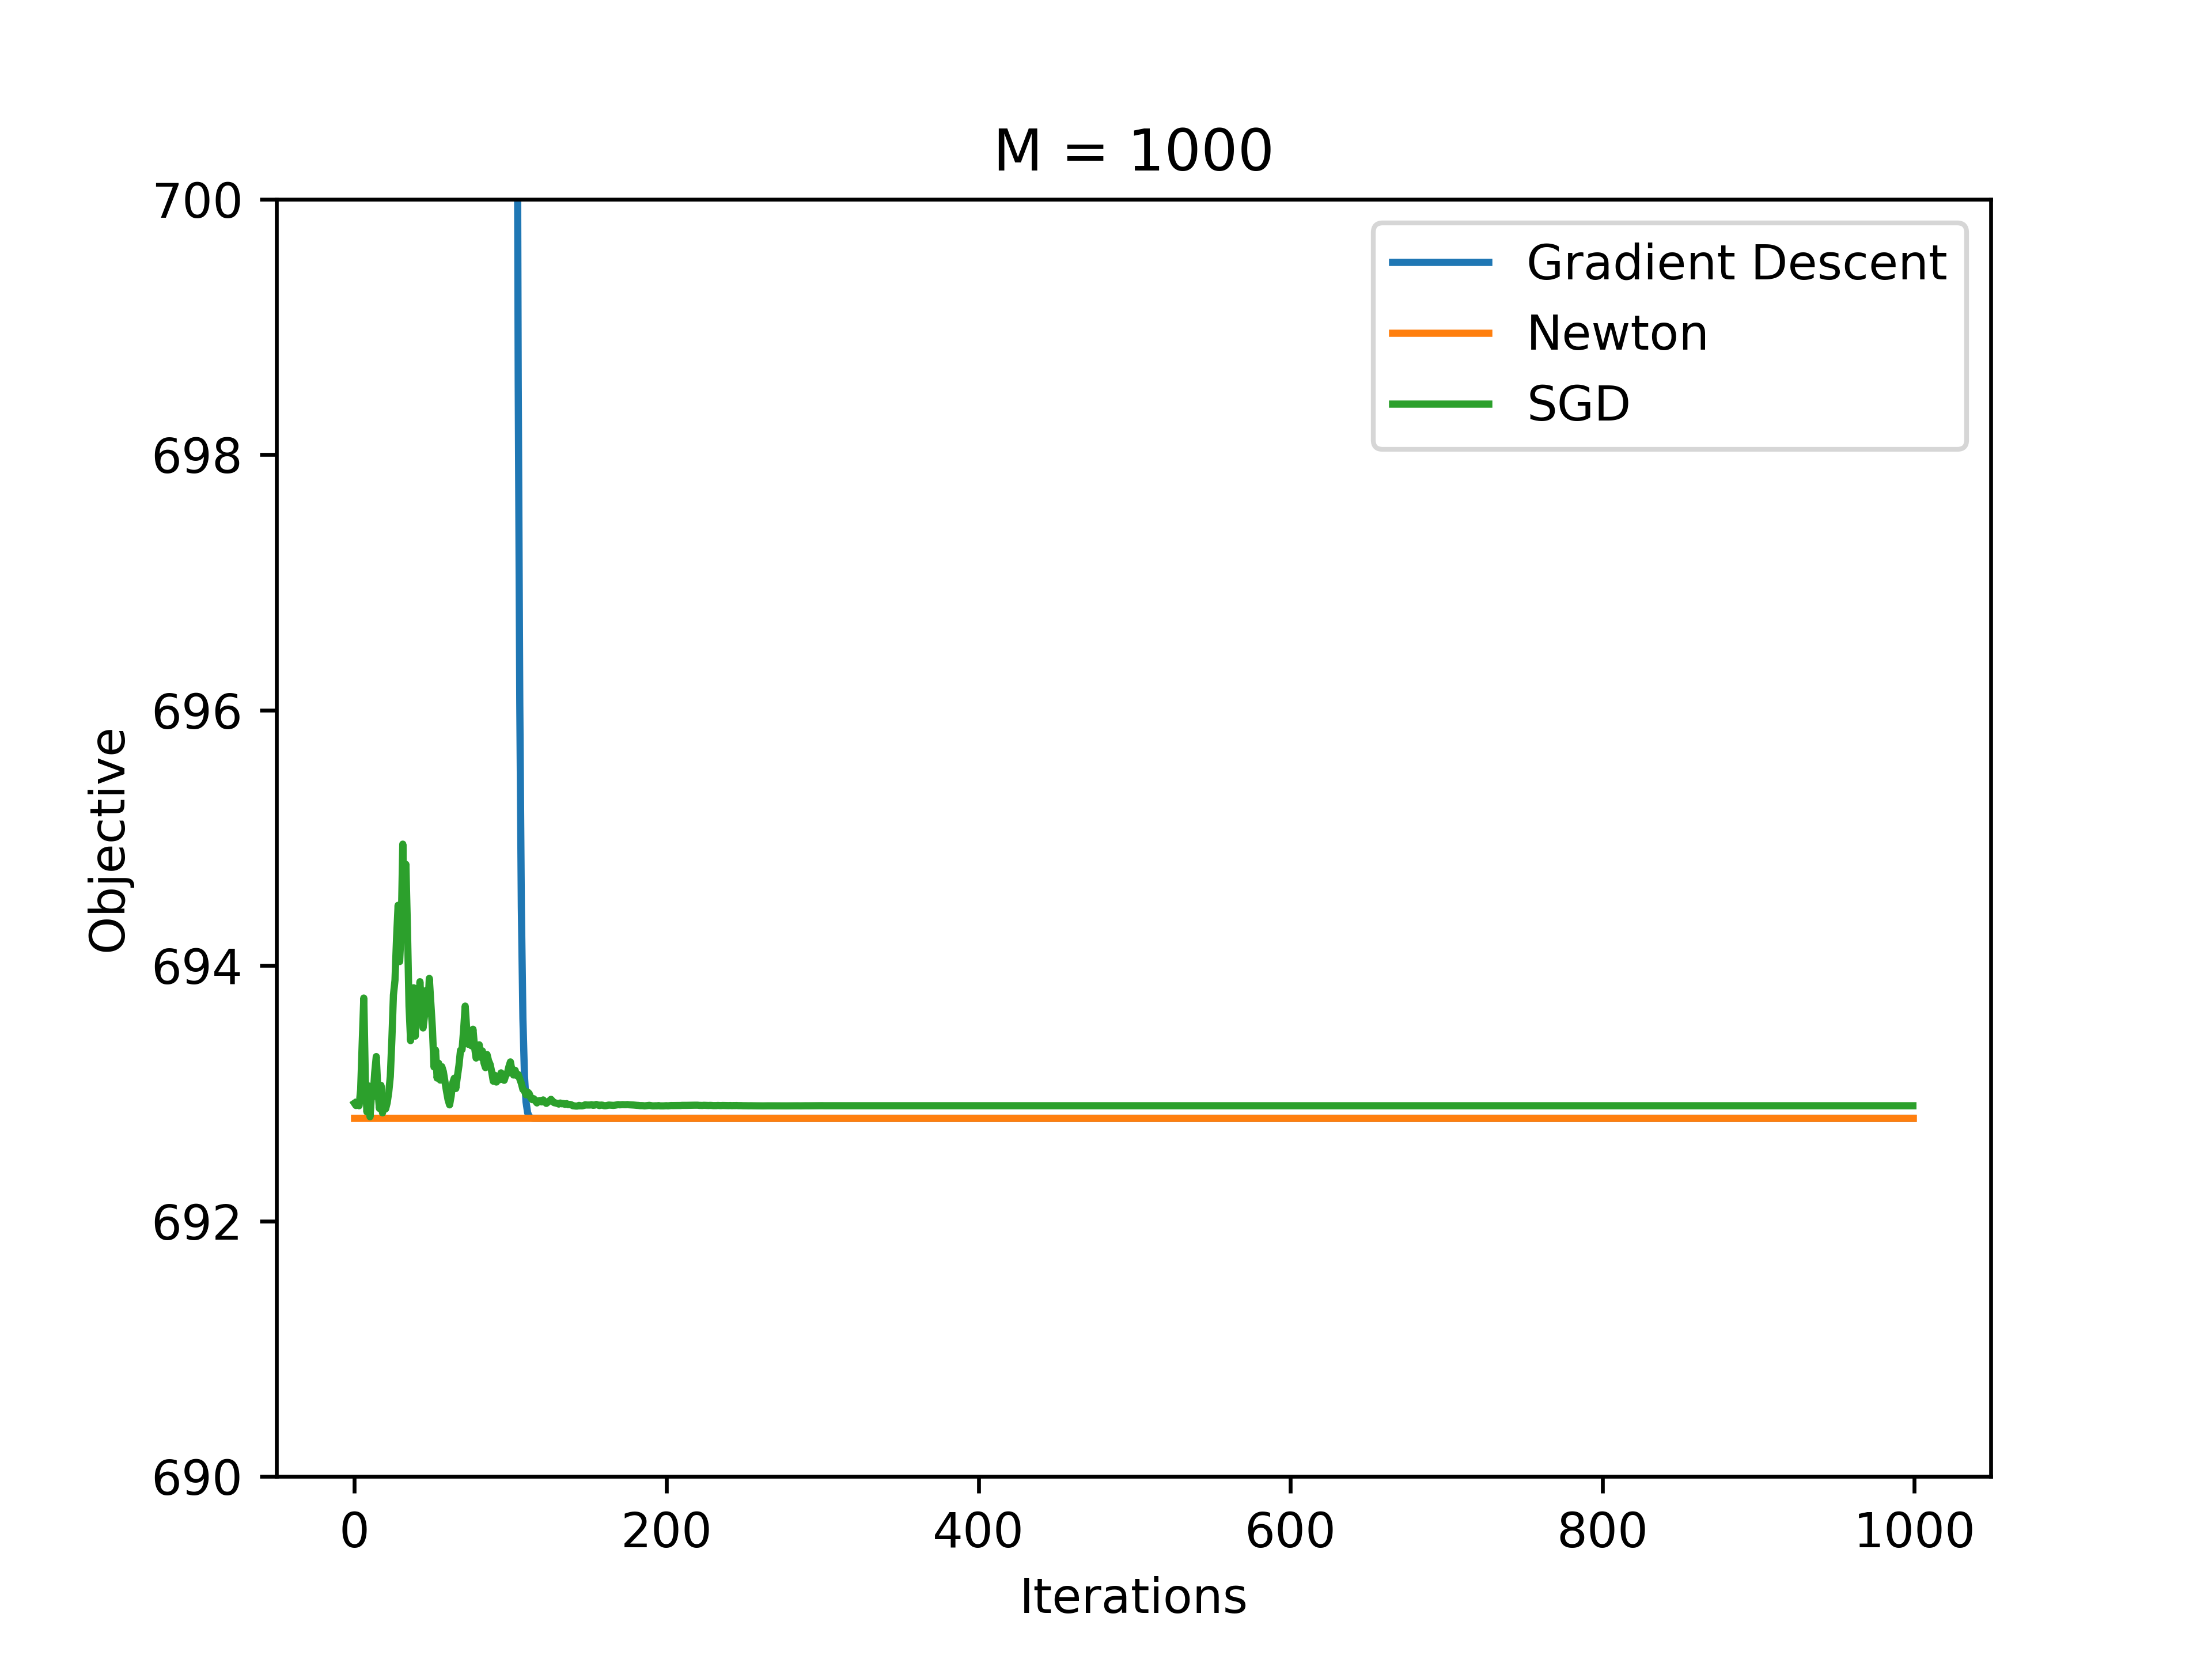
\includegraphics[scale=.55]{norm_m_1000.png}\\
Time per iteration\\
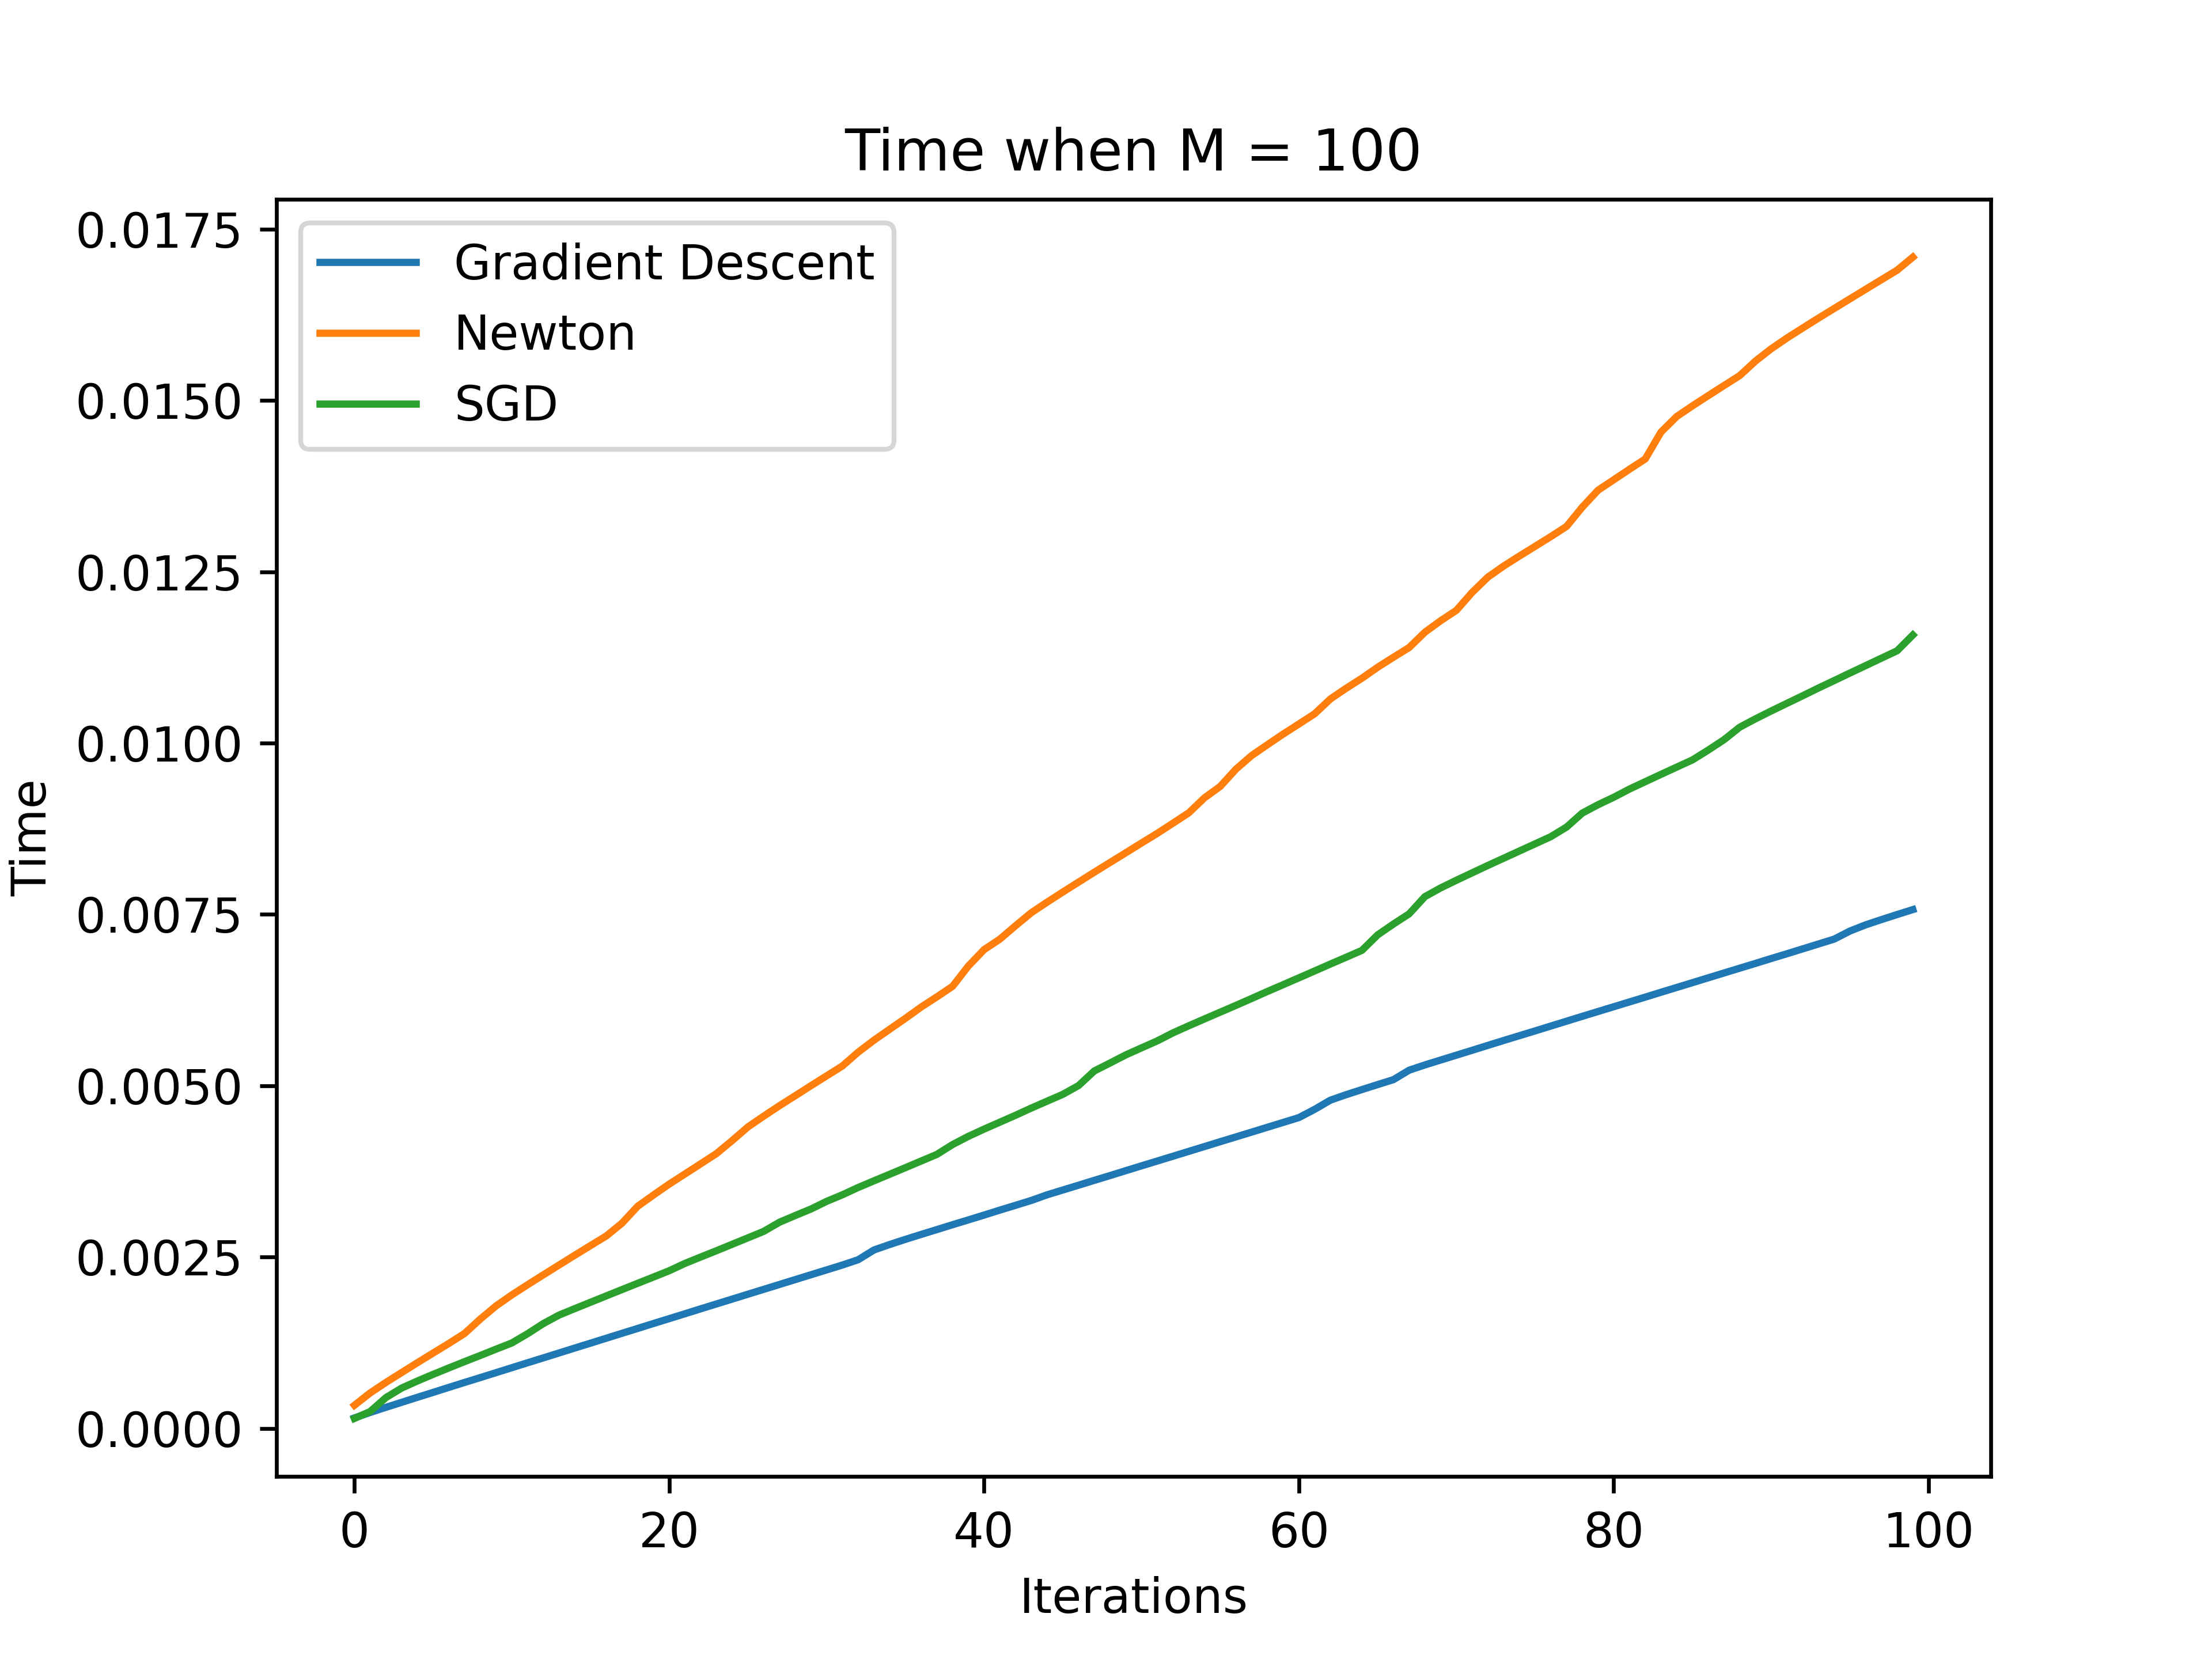
\includegraphics[scale=.55]{time_m_100.png} & 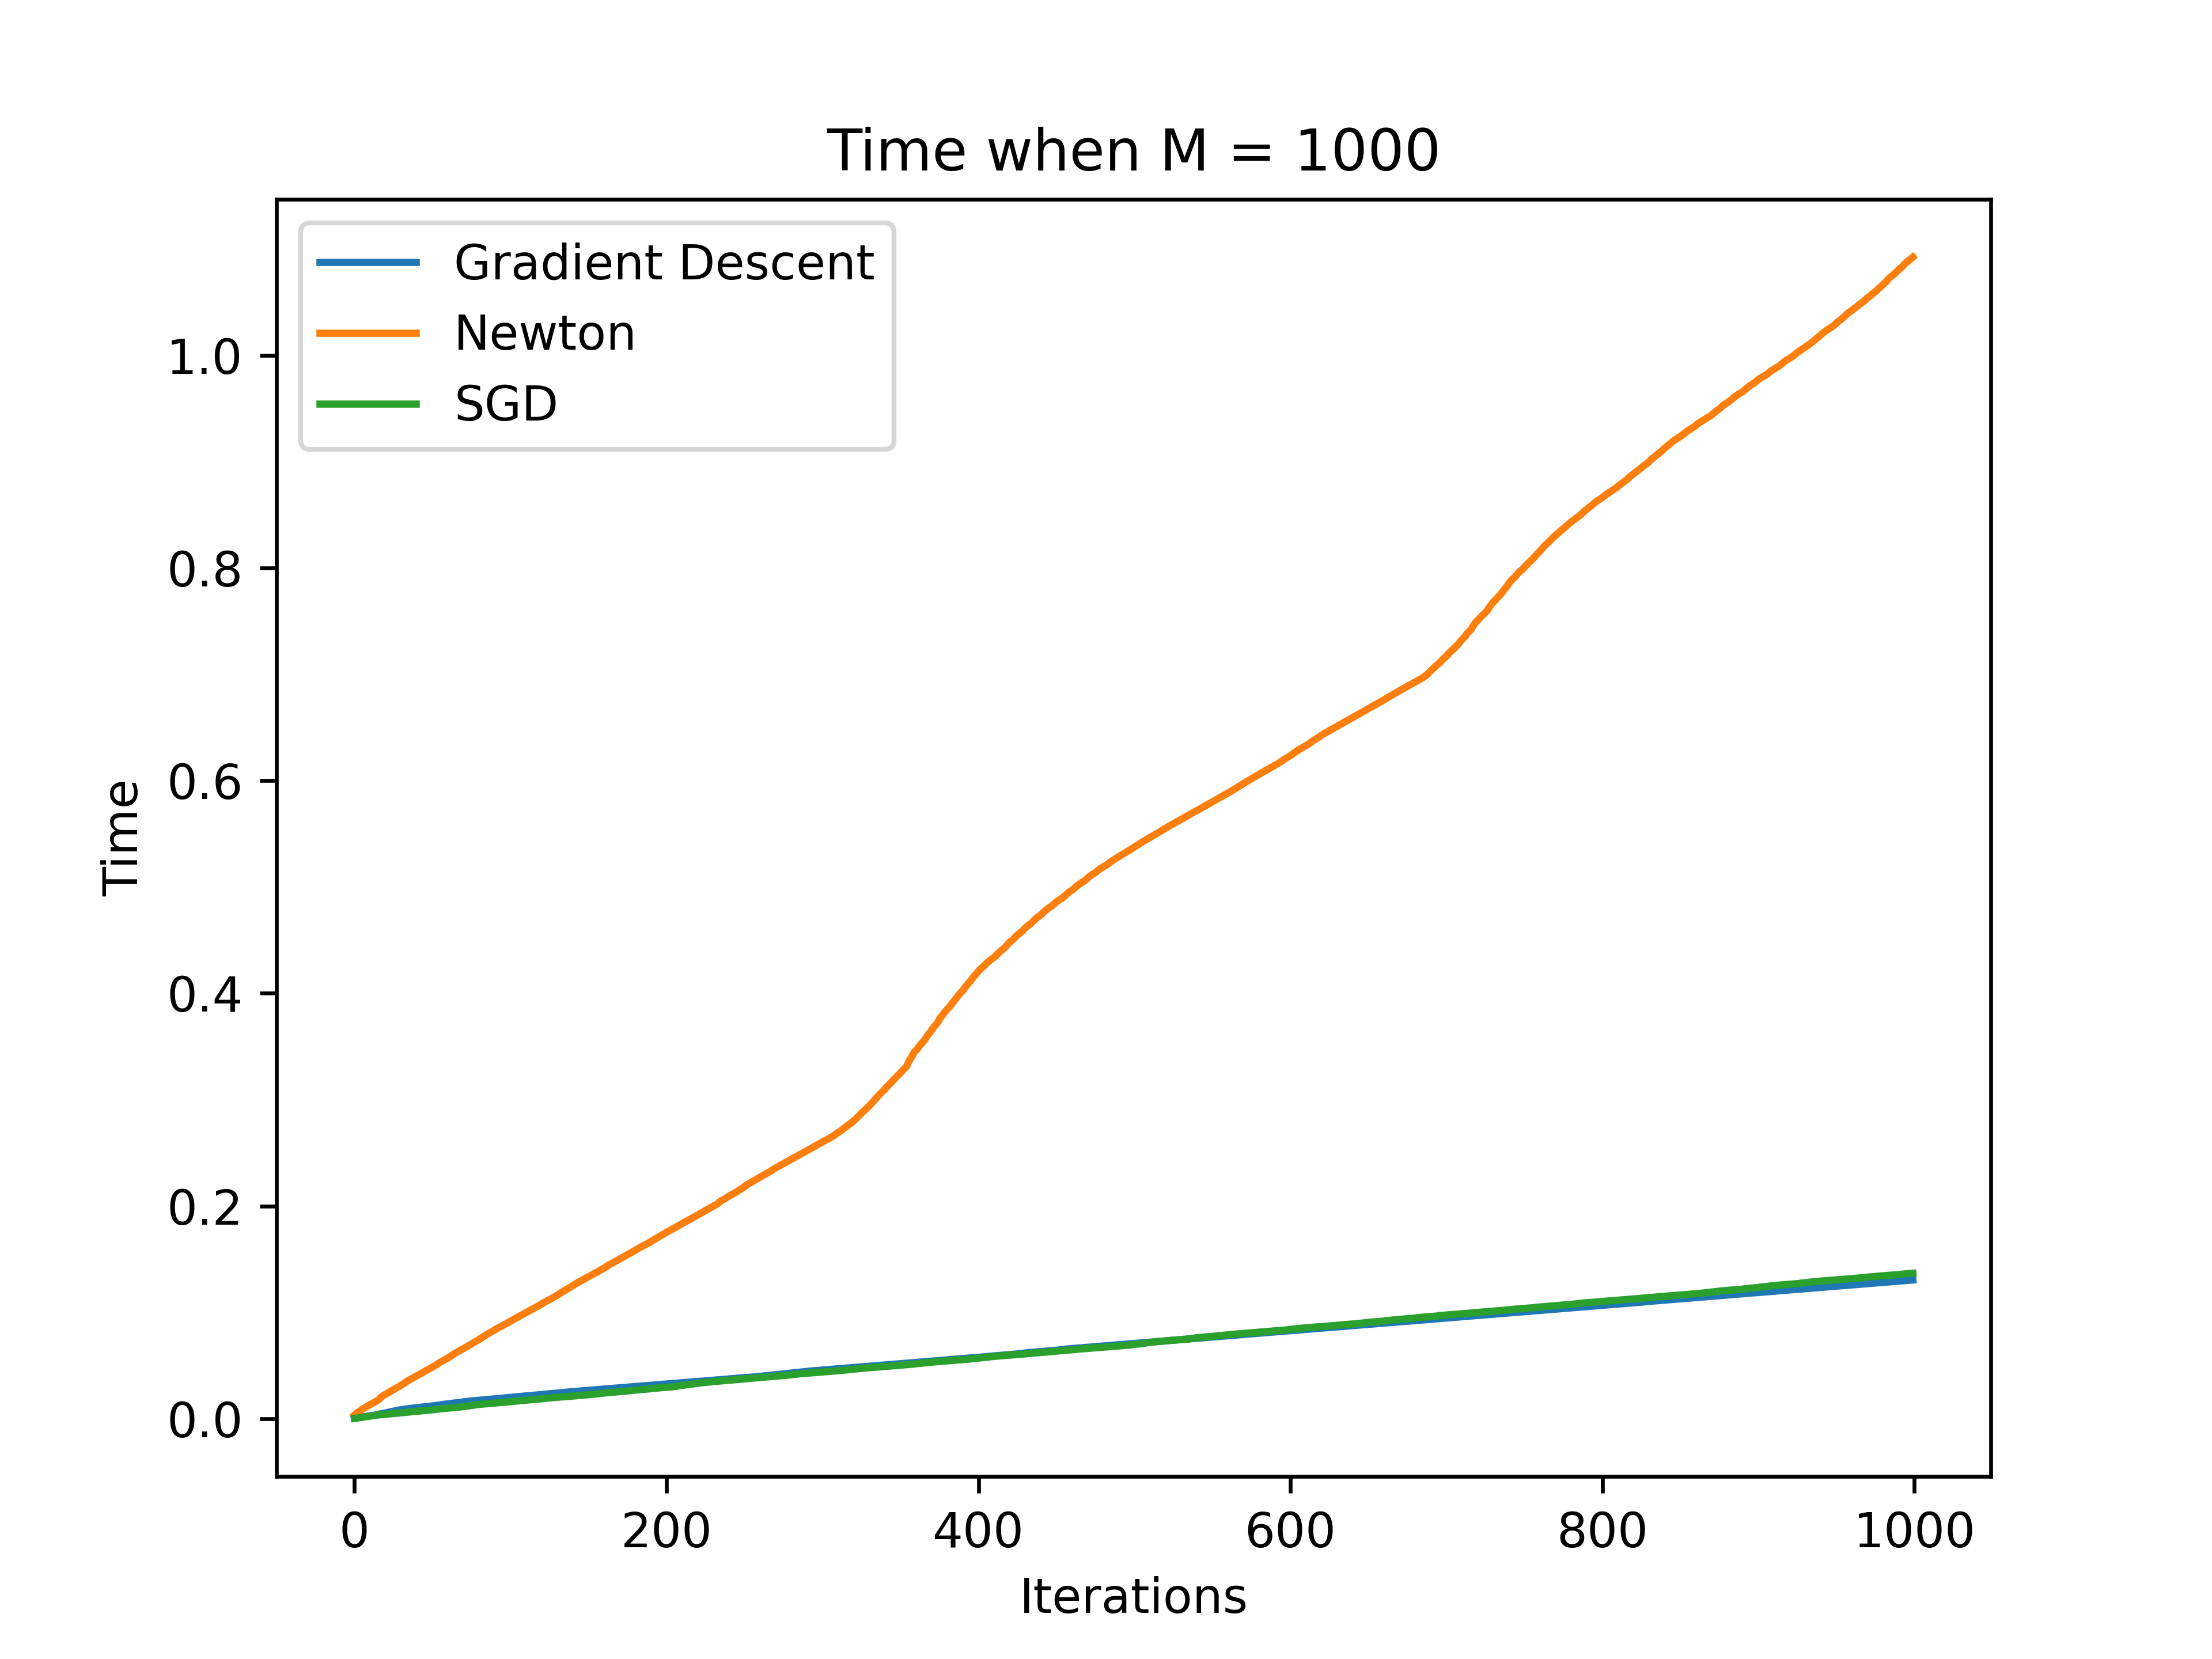
\includegraphics[scale=.55]{time_m_1000.png}
\end{tabular}

There are several observations I made from these graphs.\\\\
First I see that SGD does not converge, while is this unusual it is not expected to converge since the batch size is 1 and I am taking the gradient of 1 random training sample. This wouldn't matter as much however x and y are randomly generated with no specific pattern. Therefore the gradient of 1 point may be very different from the gradient of another. When M = 1000 Gradient descent appears from the top and quickly converges to 0. I found that in the beginning the Norm is in the 3000s and then it starts to converge. I believe this is because with a higher training set there is room for higher error. I also noticed that for all random data, the best $\beta$ was normally not far from [0, 0],from my understanding this is because none of the data has any real world pattern since it is all randomly generated. Because of the close intial guess, Newton's method converge within $<$ 5 iterations which does not appear on the graphs.  \\\\

When M = 100 Newton's method takes the longest unsurprisingly, however SGD takes 5 milliseconds longer than Gradient Descent. I believe that in this case the extra line of code in the SGD gradient calculation creating a random number accounts for this difference as I am calling an external function. This hypothesis is further justified as SGD is narrowly faster than Gradient Descent when M = 1000. Therefore I believe when M is Larger SGD will be faster than Gradient Descent, and at that time Newton's method would outlive the entire human race with how long it would take to calculate. \\\\

My code is at the bottom of exam, I didn't include the plot code as it is just plotting the data. 
\newpage
\section*{Problem 7 [10 pts]}
Please design an (either toy or real-world) experiment  to demonstrate that PCA can be helpful for denoising.\\
In my experiment I took the Lenna image and an image from the MNIST dataset. I then added noise to it and performed PCA by SVD of the first 50 columns of each image. Code will be included at end of exam. \\
\begin{tabular}{c c c}
Original Image & 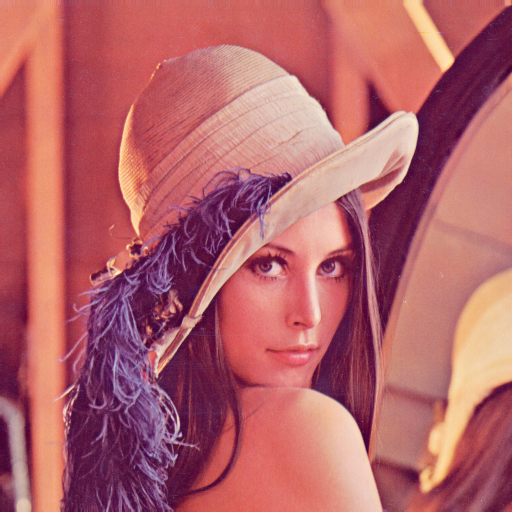
\includegraphics[scale=.3]{Lenna.png} & 
\includegraphics[scale=.3]{3.png}\\
Image with noise & 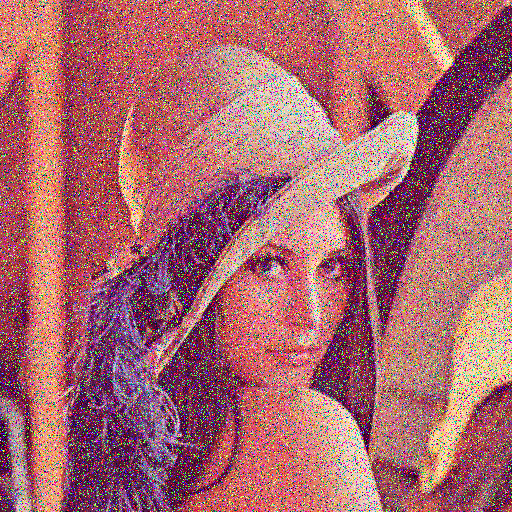
\includegraphics[scale=.3]{Lenna_noise.png} & 
\includegraphics[scale=.3]{3_noise.png}\\
Image with reduced noise by PCA & 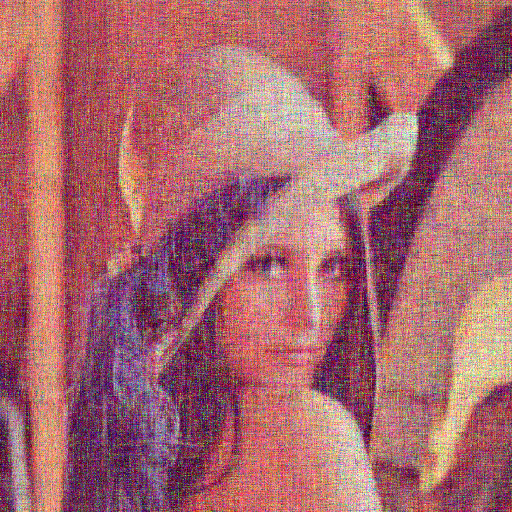
\includegraphics[scale=.3]{Lenna_reduced_noise.png} & 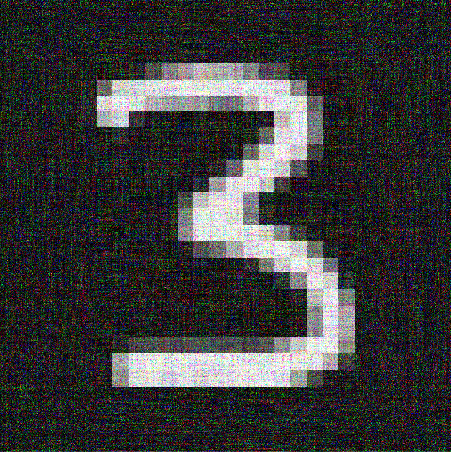
\includegraphics[scale=.3]{3_reduced_noise.png}\\
\end{tabular}
\newpage
\section*{Bonus Problem 8 [10 pts]}
\begin{equation}
	\text{\bf Solve:} \quad \min \|\vx\|_{0} \quad \mbox{s.t.}\quad { \mA \vx = \vy. }
\end{equation}
We have proved that if $\vy = \mA \vx_o$ with
\begin{equation}\label{krank}
	\|\vx_o\|_0 \; \le \; \tfrac{1}{2} \, \mathrm{krank}(\mA).
\end{equation}
Then $\vx_o$ is the unique optimal solution to the  $\ell^0$ minimization problem\index{$\ell^0$ minimization}
\begin{equation}
	\min \|\vx\|_{0} \quad \mbox{s.t.}\quad { \mA \vx = \vy. }
\end{equation}
However, when $\mA$ is of size $5 \times 12$, the following figure illustrates the fraction of success across 100 trials.
\begin{figure}[h!]
	\centering
	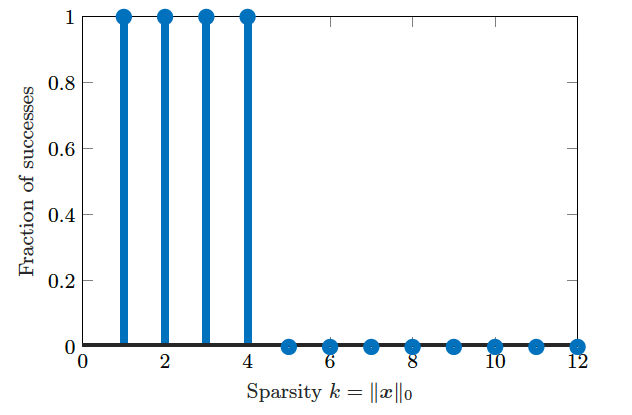
\includegraphics[width=7cm]{simulation-L0.png}
	% \caption{Caption}
	% \label{fig:my_label}
\end{figure}    
Apparently $krank(\mA)\le rank(\mA)\le 5$, therefore, when sparsity $k=1, 2$ satisfying Eq. (\ref{krank}) it has $100\%$ recovery success rate is not surprising. However, the above experiment also shows even $k=3, 4$ which violates Eq. (\ref{krank}), still it can be recovered at $100\%$. Please explain this phenomenon.\\\\
\textbf{Proof:}
\begin{equation}
A\hat{x} = y \rightarrow A(\hat{x} - x_0) = A\hat{x} - Ax_0 = y - y = 0
\end{equation}\\\\


This phenomenon can be explain because while the data theoretically cannot be recovered in the $\ell^0$ norm, it can be recovered in the $\ell^1$ norm. While $\ell^0$ is not convex, $\ell^1$ is and can be used as a convex surrogate for $\ell^0$. $|x|$ is the convex envelope for $||x||_0$. We know from experimental results like the one above that $\ell^1$  minimization succeeds with very high rate whenever the constants of n/m and k/m are relatively small. Here we introduce the Restricted Isometry Property (RIP) of order $k$ with constant $\delta \in$ [0, 1) if 
\begin{equation}
\forall \; \textbf{x} \;k-sparse,\;\; (1 - \delta)||x||^2_2 \leq ||\textbf{Ax}||^2_2 \leq (1 = \delta)||x||^2_2
\end{equation}\\
For $\ell^0$ norm, we say that $y = Ax_o$, with $k = ||x_o||_0$. If $\delta_{2k}(A) < 1$, then $x_o$ is the unique optimal solution to
\begin{equation}
min ||x||_0 \;\;\; s.t. \; Ax = y
\end{equation}\\
We can prove this by contradiction, let's say there exist an $x' \neq x$ with $||x'||_o \leq k$ Then
$x_o \: - \:x' \in null(A)$, and $||x_o - x'||_0 \; \leq 2k$. This implies that $\delta_{2k}(A) \geq 1$, contradicting our statement and therefore we can conclude the original statement is correct.\\\\
For $\ell^1$ norm recovery under RIP, we say that $y = Ax_o$, with $k = ||x_o||_0$. If $\delta_{2k}(A) < \sqrt{2} - 1$, then $x_o$ is the unique optimal solution to:
\begin{equation}
min ||x||_1 \;\;\; s.t. \; Ax = y
\end{equation}\\
Candes and Tao proved in 2006 originally that $\delta_{2k} < \sqrt{2} - 1$\\\\
Computing the RIP constant $\delta_k(A)$ is an np-hard problem, however we know that there exists a numerical constant C $>$ 0 such that if $A \in \mathbb{R}^{mxn}$ is a random matrix with entries independent $\mathcal{N}(0, \frac{1}{m})$ random variables, with high probability, $delta_k (A) < \delta$, provided that
\begin{equation}
m \geq Ck\: log(n/k) / \delta^2
\end{equation}\\
With incoherence, we need $m \geq \Omega (k^2)$. Here this result allows (k,m,n) to scale proportionally: $m \geq \Omega (k)$.
\newpage
\section{Code}
\subsection{Minmize Elastic Net Objective Problem 1}
\lstinputlisting{problem_1.m}
\subsection{Minimie Objective Problem 5}
\lstinputlisting{problem_5.m}
\lstinputlisting{objective_p5.m}
\subsection{Logistic Regression Problem 6}
\lstinputlisting[language=python]{logistic_reg.py}
\subsection{Denoise Problem 7}
\lstinputlisting{denoise.m}
\end{document}
